\chapter{Development}
% [Description of methods used (e.g., Checkstyle, PMD, Javadoc) AND any additional libraries that you used]

For this project, the program was written using the esp-idf. Which is an 
open-source driver library for the esp32 which is the micro-controller that is
being used for this project because of its low cost and built-in WI-FI
and MQTT capabilities.

To check the style of the code cpplint was used. This is based on the Google C++ style guide. 
To check for static analysis errors CppCheck was used. To generate documentation Doxygen was used.

\section{Code Standards}
% [Include report on code standards and justification for any variances]
The following is a copy of the output from cpplint. The errors are about copyright 
information not being included in the file. This is due to there not being any 
copyright information yet on this project as it is still in development and not 
intended for release. 

The other error is not including the directory when naming
header files. This is due to the compiler finding the required files in the esp-idf
that controls the building and flashing of the program. Therefore no directories can
be included in this method.
\begin{tiny}
\begin{verbatim}
main/lock_main.c:0:  No copyright message found.  You should have a line: "Copyright [year] <CopyrightOwner>"  [legal/copyright] [5]
main/lock_main.c:8:  Include the directory when naming header files  [build/include_subdir] [4]
main/lock_main.c:9:  Include the directory when naming header files  [build/include_subdir] [4]
main/lock_main.c:10:  Include the directory when naming header files  [build/include_subdir] [4]
main/lock_main.c:11:  Include the directory when naming header files  [build/include_subdir] [4]
main/lock_main.c:12:  Include the directory when naming header files  [build/include_subdir] [4]
main/lock_main.c:13:  Include the directory when naming header files  [build/include_subdir] [4]
main/lock_main.c:14:  Include the directory when naming header files  [build/include_subdir] [4]
main/lock_main.c:15:  Include the directory when naming header files  [build/include_subdir] [4]
main/lock_main.c:27:  Include the directory when naming header files  [build/include_subdir] [4]
main/lock_main.c:28:  Include the directory when naming header files  [build/include_subdir] [4]
Done processing main/lock_main.c
Total errors found: 11
\end{verbatim}
\end{tiny}

\section{Static Analysis}
% [Include report on static analysis and justification for any variances]

\begin{figure}[htb]
    \begin{center}
        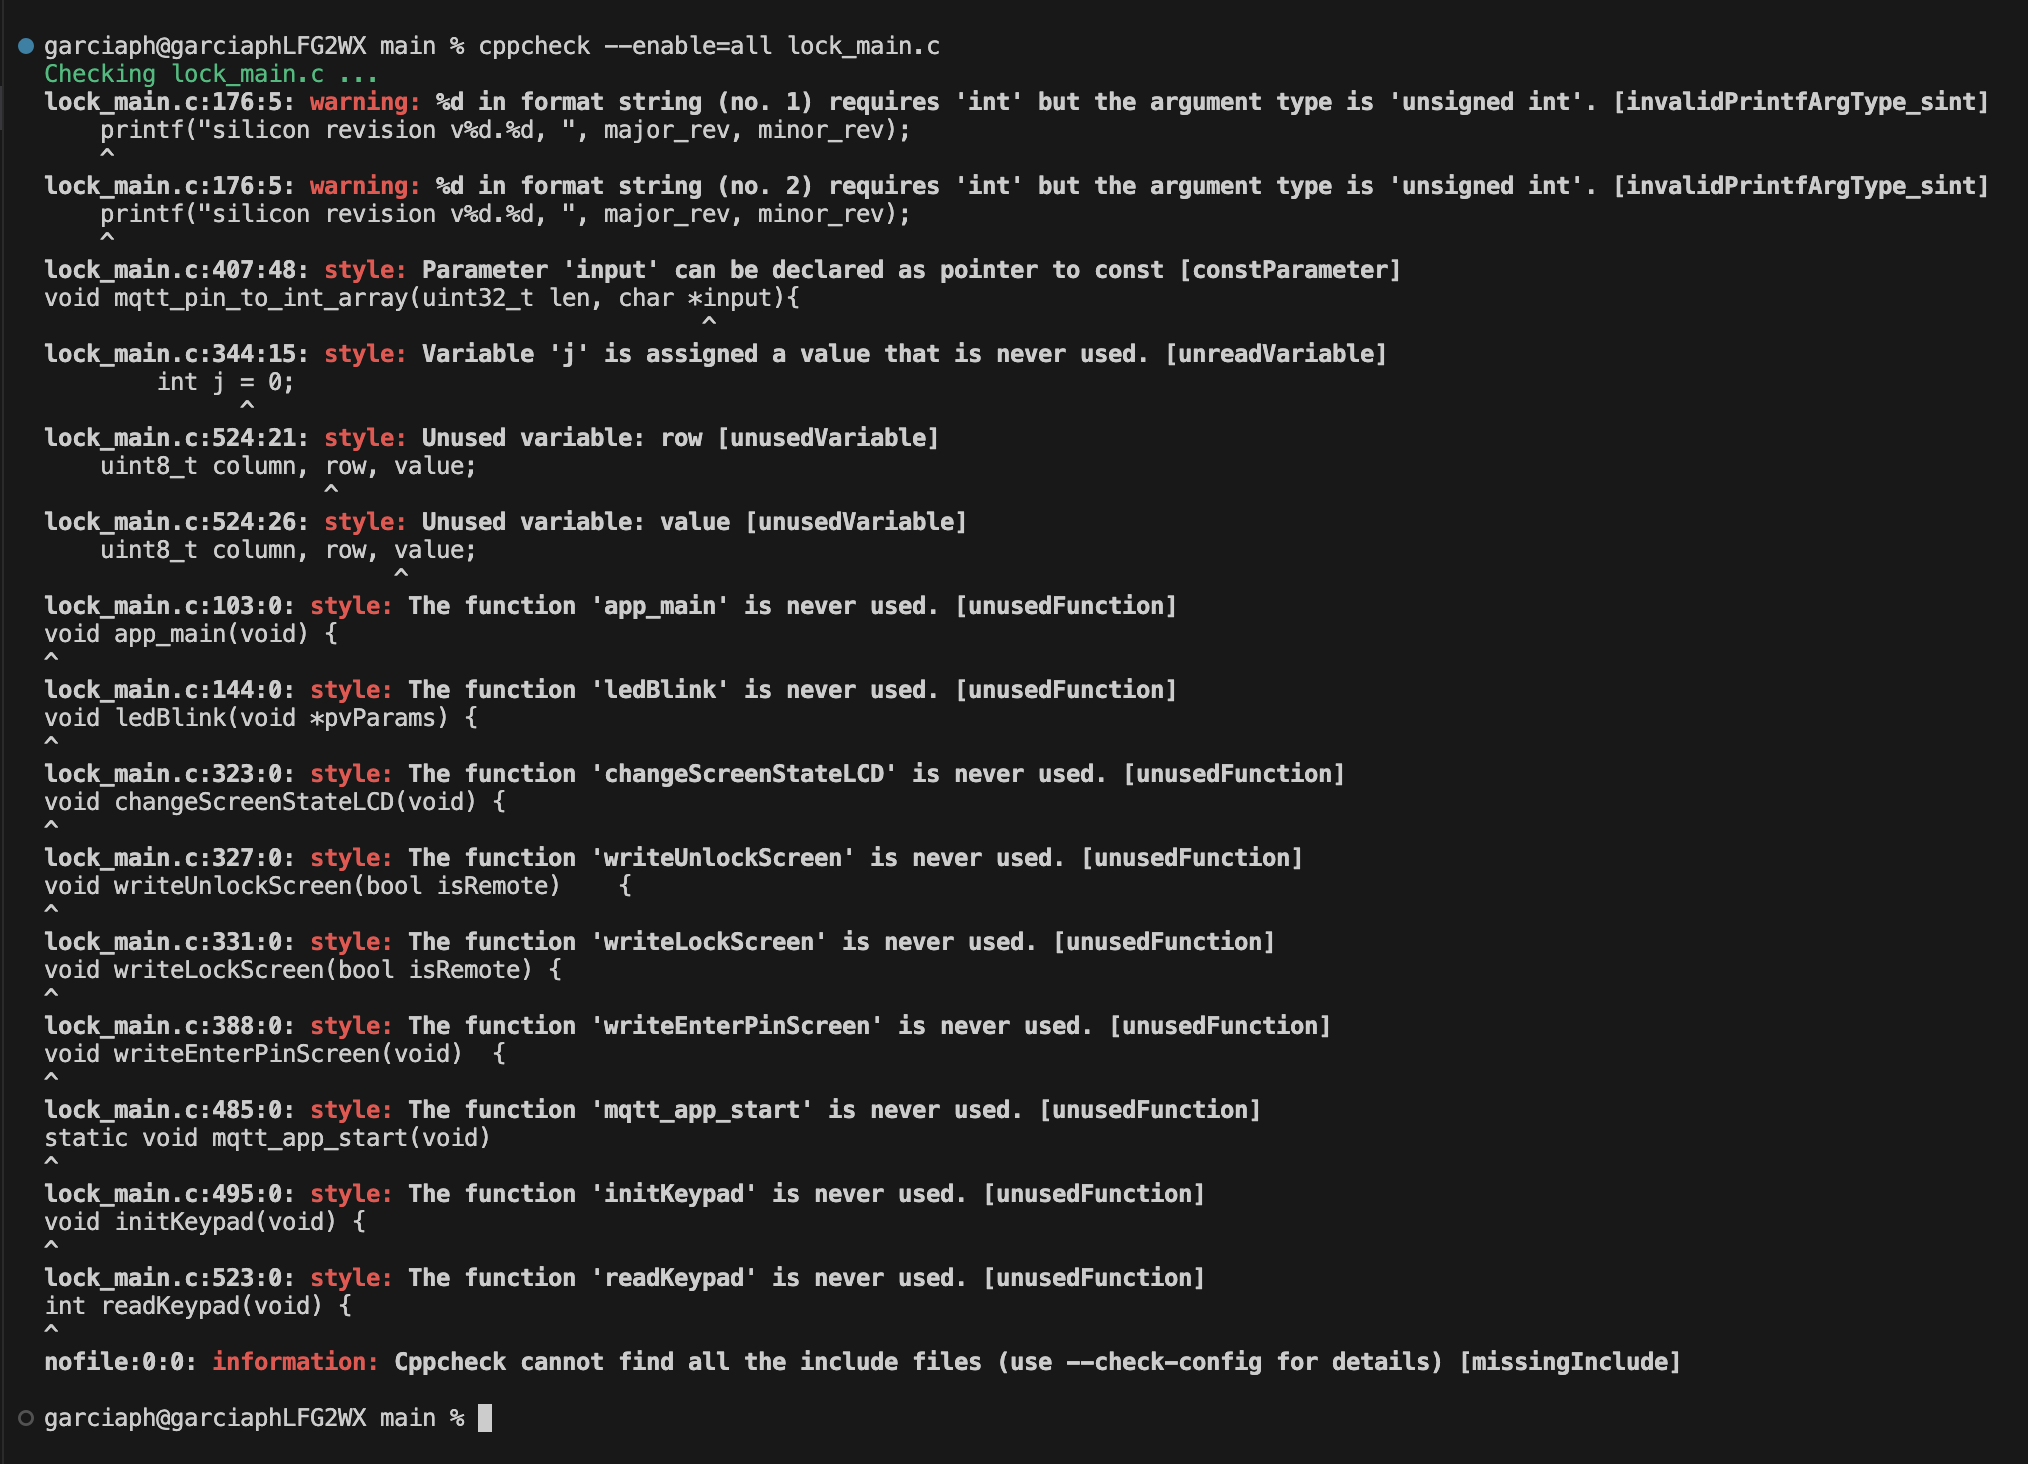
\includegraphics[width = \textwidth]{Images/CIS 350 - Project - Static Analysis Results.png}
        \caption{Static Analysis Results}
        \label{fig: Static Analysis Results}
    \end{center}
\end{figure}

The first three warnings refer to imported code that was used to verify the functionality of the selected microcontroller (MCU), ESP32. The print statements that caused the warnings will be removed. 

As for the unused function warnings, the development for some of our peripherals were started, but not completed. Once complete, the majority of the style warnings will not be reported again. 

\clearpage
\section{Code Documentation}
\subsection{Main System Documentation}
% [Include link to javadocs (likely included as separate file) and justification for any non-documented areas]
For the main system, Doxygen was used to generate the code documentation. The link to the Doxygen output is \href{https://github.com/CIS-350/lock/blob/development/html/release_1_doxygen.pdf}{here}.

\subsection{Mobile App Documentation}
For the mobile application, the project is going to be documented using DartDocs.

\section{Configuration Management}
% [Include link to Git repository and Git log] 
% [Explain / describe method for tracking releases]
The GitHub repository for the main system code base can be viewed \href{https://github.com/CIS-350/lock}{here} and the code base for the mobile lock app can be viewed \href{https://github.com/CIS-350/lock_app}{here}. In both repositories, the release specific to the midterm is labeled as "Midterm Release".\\
\\
A log containing all of the commits made to the main code base can be viewed in \hyperlink{mainlog}{\color{blue}{Appendix 8.1}} and the commits for the mobile application code base can be viewed in \hyperlink{applog}{\color{blue}{Appendix 8.2}}.\\
\\
For the project up until this point, code releases have been tracked by branching off of main for development, and merged back into main through pull requests after code development is finished. From there, a release on GitHub is created. After this midterm release however, we plan on implementing a dedicated development branch that we will be able to push changes to while still maintaining a stable code base in the main branch.
